\documentclass[a4paper]{article}
\usepackage[14pt]{extsizes}
\usepackage{fontspec} 
\defaultfontfeatures{Ligatures={TeX},Renderer=Basic} 
\setmainfont[Ligatures={TeX,Historic}]{Times New Roman}
\usepackage[english, russian]{babel}
\usepackage{setspace}
\usepackage{indentfirst}
\usepackage{graphicx}
\usepackage[top=2cm, bottom=2cm, left=3cm, right=1cm, nofoot, nohead]{geometry}
\linespread{1.3}
\setlength{\parindent}{1.25cm}
\bibliographystyle{plain}
\renewcommand{\contentsname}{Оглавление}
\counterwithin{figure}{section}
\setlength{\footskip}{25pt}
\newcommand{\anonsection}[1]{\section*{#1}\addcontentsline{toc}{section}{#1}}
\newcommand{\numsection}[1]{\section*{#1}\addcontentsline{toc}{section}{#1} \refstepcounter{section}}
\begin{document}
	\begin{titlepage}
		\begin{center}
			~~~
			\\
			~~~
			\\
			~~~
			\textbf{МИНИСТЕРСТВО ОБРАЗОВАНИЯ РЕСПУБЛИКИ БЕЛАРУСЬ\\
			БЕЛОРУССКИЙ ГОСУДАРСТВЕННЫЙ УНИВЕРСИТЕТ\\
			МЕХАНИКО-МАТЕМАТИЧЕСКИЙ ФАКУЛЬТЕТ\\
			Кафедра теоретической и прикладной механики\\}
			~~~
			\\
			~~~
			\\
			~~~
			\\
			~~~
			Шевелёв Дмитрий Юрьевич\\
			~~~
			\\
			~~~
			\textbf{ВЛИЯНИЕ ВИХРЕГЕНЕРАТОРОВ В ТУРБУЛЕНТНОМ ПОГРАНИЧНОМ СЛОЕ НА ЛОКАЛЬНОЕ ТРЕНИЕ И ПЕРЕНОС\\}
			~~~
			\\
			~~~
			\\
			~~~
			Дипломная работа\\
			~~~
			\\
			~~~
			\\
			~~~
		\end{center}
		\begin{flushright}
			Научный руководитель:\\
			кандидат физико-математических наук,\\
			доцент А. Д. Чорный\\
		\end{flushright}
		\begin{flushleft}
			Допущен к защите\\
			<<$\underline{\hspace{1cm}}$>>$\underline{\hspace{3cm}}$ 2023 г.\\
			Зав. кафедрой теоретической и прикладной механики\\
			доктор физико-математических наук, профессор М. А. Журавков
		\end{flushleft}
		~~~
		\\
		~~~
		\begin{center}
			Минск, 2023
		\end{center}
	\end{titlepage}
	\tableofcontents
	\newpage
	\anonsection{Перечень условных обозначений}
	\noindent\textbf{LES} -- Large eddy simulation, метод моделирования крупных вихрей\\
	\textbf{SGS} -- Sub grid scale, модели подсеточного масштаба
	\newpage
	\anonsection{Введение}

		Турбулентные пограничные слои развиваются на поверхностях многих инженерных конструкций: от теплообменных устройств, элементов воздушно-реактивных двигателей до планеров самолетов, корпусов кораблей и крупных строительных сооружений. Они определяют как сопротивление трения, так и перенос тепла. Вихревая структура этих слоев открывает возможность ее изменения путем воздействия на процесс формирования вихрей. 
		
		Одним из способов управления и уменьшения потерь энергии в турбулентном пограничном слое является использование методов активного и пассивного контроля турбулентности, например, установка поперечных ребер на поверхности или введение потока тепла в стенки. Более глубокое понимание особенностей турбулентного пограничного слоя может помочь снизить энергетические затраты и повысить эффективность различных технологий.
		\newpage
	\numsection{Глава 1}
	\subsection{Структура пограничного слоя}
		Пограничный слой -- область течения вязкой жидкости (газа) с малой по сравнению с продольными размерами поперечной толщиной, образующаяся у поверхности обтекаемого твёрдого тела или на границе раздела двух потоков жидкости с различными скоростями или температурами. Пограничный слой характеризуется резким изменением в поперечном направлении скорости (динамический пограничный слой) или температуры (температурный пограничный слой).
		
		На формирование течения в пограничном слое основное влияние оказывают вязкость, теплопроводность и диффузионная способность жидкости. Внутри динамического пограничного слоя происходит плавное изменение скорости от её значения во внешнем потоке до нуля на стенке вследствие прилипания вязкой жидкости к твёрдой поверхности. Аналогично внутри пограничного слоя плавно изменяется температура.\\		
	\begin{figure}[h]
		\centering
		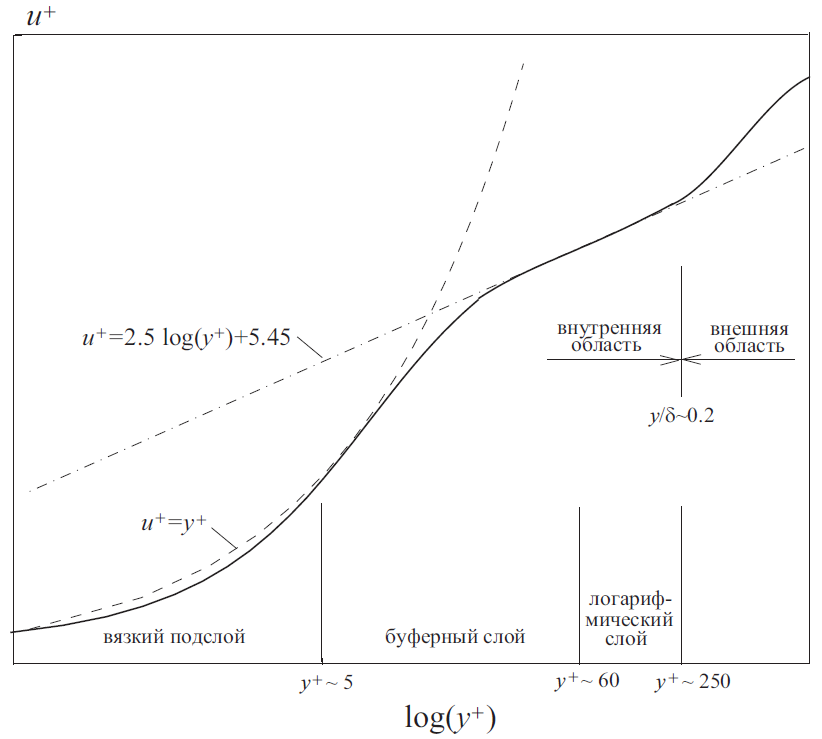
\includegraphics[width=0.7\linewidth]{../Assets/ПогранСлой}
		\caption{Схема слоя}
	\end{figure}
		
		Турбулентный пограничный слой разделяется на две области: внешняя и внутрення. Внутренняя область пограничного слоя занимает примерно 20\% от толщины всего слоя и в ней генерируется до 80\% энергии турбулентности.
		
	\subsubsection{Внешняя область}
		
		Внешний слой является областью полностью развитого турбулентного течения, в котором распределение скорости описывается логарифмическим законом. Полное затухание возмущений во внешней области происходит на расстоянии, во много раз превышающем линейный масштаб турбулентности.
		‍
		
		Чтобы определить поток во внешней зоне, применяют фильтрованные или усредненные по Рейнольдсу уравнения Навье-Стокса. В то же время, профиль скорости во внутренней зоне сравнительно мало зависит от различных внешних условий, таких как числа Рейнольдса и градиент давления, что позволяет использовать универсальные соотношения (пристеночные функции) для связи параметров потока с расстоянием от стенки. Этот метод также базируется на гипотезе о локальном равновесии энергии турбулентных пульсаций и свойствах локальной изотропности диссипирующих вихрей.
		
	\subsubsection{Внутрення область}
	
		Вязкий подслой, буферный и логарифмический слои составляют внутреннюю область пограничного слоя. Она характеризуется высокой скоростью переноса массы, импульса и тепла, что приводит к повышенной трению и потере энергии.
		
		‍
		Существует два подхода к моделированию течения в пристеночной области. В первом подходе используются полуэмпирические формулы (пристеночные функции) для описания внутреннего слоя потока, в то время как во втором подходе модели турбулентности модифицируются таким образом, чтобы разрешать всю пристеночную область потока, включая вязкий подслой, при условии обеспечения необходимого разрешения сетки в пограничном слое. Такие модели турбулентности могут быть использованы для расчета турбулентных течений во всей расчетной области (включая пристеночную область течения).
	\subsection{Турбулентное состояние пограничного слоя}
	‍
		Турбулентное движение в пограничном слое возникает из-за нестабильности потока, которая проявляется в виде вихрей различных размеров и интенсивности. Эти вихри перемешивают слои жидкости или газа, что приводит к увеличению переноса массы и энергии вдоль поверхности твердого тела. Параметры турбулентного потока в пограничном слое характеризуются такими величинами, как скорость, давление, плотность и температура. Важными параметрами являются также коэффициент трения, переноса тепла и массы. Турбулентное течение с большим числом Рейнольдса называют развитой турбулентностью.
		
		Для описания турбулентности используются уравнения Навье-Стокса, которые описывают законы сохранения массы, импульса и энергии для жидкости. Однако аналитическое решение этих уравнений возможно только для очень простых течений. В общем случае для описания турбулентных потоков применяются численные методы, такие как метод прямого численного моделирования или моделирование крупных вихрей. Одной из фундаментальных проблем гидродинамики турбулентных течений является проблема турбулентного переноса. Она связана с необходимостью описать перемещение частиц жидкости и массы, энергии и импульса в условиях сложных турбулентных потоков
		
		Существует каскадный перенос энергии, т.е. её передача от более крупных вихрей к более мелким. Наиболее крупные вихри получают энергию от осредненного течения, передают её всё более мелким, а наиболее мелкие диссипируют в тепло. Скорость этого процесса в силу хаотичности природы турбулентности также колеблется вокруг некой величины, при этом ее мгновенное значение может становиться отрицательным. Иными словами, в некоторые моменты времени энергия может передаваться от более мелких вихрей к более крупным, но эта флуктуация компенсируется более интенсивной передачей энергии по каскаду в другие моменты времени.
		
		
	\subsection{Локальное трение и перенос}
	
		% Тут надо ещё подумать почитать и переделать %
		Локальное трение - это сопротивление движению тела, возникающее при контакте поверхностей, на которых оно скользит. В отличие от идеального или нулевого трения, локальное трение всегда присутствует в реальных условиях. Перенос же - это процесс перемещения чего-либо из одного места в другое. Локальное трение может оказывать влияние на перенос. Например, если объект движется по поверхности, на которой есть локальное трение, то его движение замедляется и потеря энергии происходит за счет трения. Это может привести к тому, что объект не сможет полностью передать свою энергию и импульс другому объекту при столкновении, так как часть энергии будет потеряна на трение.
	
	\numsection{Глава 2}
	\subsection{Постановка задачи}
	\subsection{Визуализация поставленной задачи}
		% Возможно это всё как подпункт для постановки задачи(либо сразу подпункт построение сетки) %
		% Тут ещё описать параметры канала и сделать контрастные скриншоты  %
	\subsubsection{Построение сети}
		% Описать построение сетки, способы и про оптимизацию + схема из отчёта + вся статистика сетки %
	\subsection{Используемый метод моделирования}
		% Может сделать как выбор модели и описать ещё и RANS(если будут результаты, прям хороший вариант для объёма) %
		Несмотря на интенсивное развитие вычислительной техники и впечатляющие успехи, достигнутые в последние годы как в области построения эффективных численных алгоритмов, предназначенных для решения задач гидромеханики и тепломассопереноса, так и в разработке сопутствующего математического обеспечения (генераторы сеток, интерактивные системы ввода данных и систем визуализации результатов расчетов), проблема численного моделирования турбулентности, как и на протяжении многих предшествующих десятилетий, по-прежнему остается одной из наиболее сложных и актуальных проблем механики жидкостей. В отличие от ламинарных течений однофазной среды (жидкости или газа), расчет которых, благодаря отмеченным выше достижениям, стал во многом рутинной процедурой, надежное предсказание характеристик сложных турбулентных течений, представляющих наибольший практический интерес все еще остается сложным.
		
		Метод крупных вихрей (LES) был предложен Иосифом Смагоринским в 1963 году. Он основан на двух предположениях. Первый предполагает, что течение можно разделить на движение крупных и мелких вихрей. Крупные вихри, находящиеся под прямым воздействием граничных условий и несущие в себе максимум рейнольдсовых напряжений, рассчитываются. Мелкомасштабная турбулентность считается изотропной и имеющей универсальные характеристики, а потому менее критичной и более поддающейся моделированию. Другой  заключается в возможности аппроксимации нелинейных взаимодействий между крупными и мелкими вихрями только по крупным вихрям с использованием подсеточных моделей(SGS). Иначе говоря, принимается гипотеза о статистической независимости крупных и мелких вихрей.
		
		Статистика крупных вихрей обычно не чувствительна к подсеточному моделированию за исключением пристеночной области. Имеющиеся подсеточные модели корректно предсказывают не только осредненные характеристики потока (первые и вторые моменты), но также и флуктуации интегральных характеристик, например, коэффициентов сопротивления и подъемной силы\cite{Fureby2000}.
		
		Мелкомасштабное движение исключается из уравнений Навье-Стокса при помощи применения операции фильтрации и моделируются с помощью подсеточных моделей. На рисунке \ref{fig:lesfilter} показан принцип работы фильтров, где $f(x)$ - исходный вариант, $\tilde{f}(x)$ - после фильтрации.\\
		\begin{figure}[h]
			\centering
			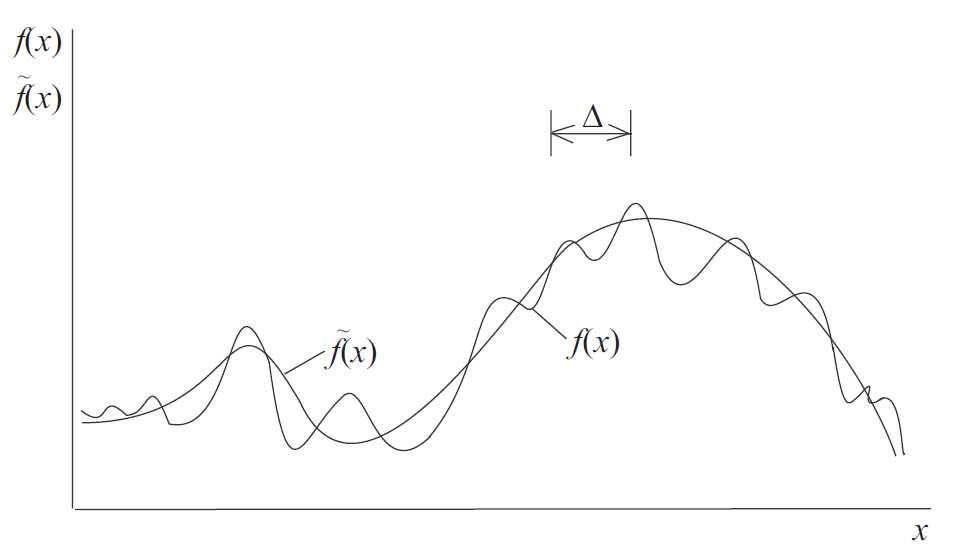
\includegraphics[width=0.7\linewidth]{../Assets/ФильтрацияLES}
			\caption{Исключение мелкомасштабных движений фильтрацией}
			\label{fig:lesfilter}
		\end{figure}
		
		Уравнение фильтра применимое к пространственно временному полю $\phi(x,t)$ представлено ниже:
		\begin{equation}
			\overline{\phi(x,t)} = \int_{-\infty}^{\infty}\int_{-\infty}^{\infty}\phi(r,t')G(x - r, t - t')dt'dr
		\end{equation}
		В данном случае $G$ - ядро изогнутости, характерное для каждого типа фильтра.
		
		Решение, полученное с помощью LES, содержит более богатую информацию по сравнению с решением на основе уравнений Рейнольдса, например, не только характеристики среднего течения (поля скорости, концентрации, температуры, давления) и распределения рейнольдсовых напряжений, но также и спектральные характеристики (спектры пульсаций скорости и давления), двухточечные моменты (например, пространственные и пространственно-временные корреляции пульсаций скорости и давления), временные и пространственные масштабы турбулентности.
	
	\subsection{Вычисление в ANSYS Fluent}
	% Тут про настройки fluent и куча его параметров при запуске вычислений %
	\numsection{Глава 3}
	\subsection{Анализ полученных результатов}
	\subsection{Влияние на локальное трение и перенос}
	\anonsection{Заключение}
	\newpage
	\addcontentsline{toc}{section}{Список использованных источников}
	\bibliography{bibliography}
\end{document}